% article_FR_4.0.tex — one-page presentation of WAC 4.0 for a DFIR magazine,
% French edition. The English edition is article_EN_4.0.tex, in this folder:
% both are maintained together, paragraph for paragraph. It follows the article
% on version 3.0 (article_FR_3.0.tex) and presents only what 4.0 adds.
%
% Build (LuaLaTeX, as the editor's recipe; build artefacts removed after):
%     ../build-docs.sh article/article_FR_4.0.tex
%
% Every figure comes from the validation and harmlessness files
% (doc/validation, doc/harmlessness) and the backlog, measured from 31 October
% to 8 November 2026 on the code of 4.0. Backlog B-061.

\documentclass[10pt,a4paper,twocolumn]{article}
\usepackage[french]{babel}
\usepackage{fontspec}
\setmainfont{Noto Sans}
\setmonofont{DejaVu Sans Mono}[Scale=0.84]
\usepackage[top=13mm,bottom=13mm,left=14mm,right=14mm,columnsep=7mm]{geometry}
\usepackage{xcolor}
\usepackage{titlesec}
\usepackage{enumitem}
\usepackage{array}
\usepackage{graphicx}
\usepackage{caption}
\captionsetup{font={small,color=gris},skip=2pt}
\usepackage[hidelinks]{hyperref}
\definecolor{marine}{HTML}{0A1A33}
\definecolor{bleu}{HTML}{2F6DB5}
\definecolor{gris}{HTML}{5B6573}
\pagestyle{empty}
\setlength{\parindent}{0pt}
\setlength{\parskip}{0.35em}
\titleformat{\section}{\color{marine}\normalsize\bfseries}{}{0em}{}
\titlespacing*{\section}{0pt}{0.7em}{0.2em}
\setlist{nosep,leftmargin=1.1em}
\newcommand{\wac}{\textsc{wac}}
\newcommand{\fichier}[1]{\texttt{#1}}
\hypersetup{pdftitle={WAC 4.0 — les serveurs Windows, l'annuaire et les sites web}}

\begin{document}

\twocolumn[{%
  {\color{marine}\LARGE\bfseries WAC 4.0 : les serveurs Windows, l'annuaire et les sites web}\par
  \vspace{0.3em}
  {\color{gris}Centre d'Excellence Cyberdéfense Aérospatiale (CEC), École de l'air et de l'espace}\par
  \vspace{0.6em}
  {\itshape Les articles consacrés aux versions 2.0 et 3.0 présentaient \wac{}
  (Windows Artefacts Collector) : un collecteur libre, en C++, qui lit les
  volumes en brut, sans rien écrire sur la machine examinée, et couvre les
  postes de XP~SP1 à Windows~11. La version 4.0 passe aux serveurs : toutes les
  générations de Server~2003 à 2025, les annuaires des contrôleurs de domaine,
  les stratégies de groupe, les serveurs web et les rôles DNS, DHCP et
  Hyper-V.}\par
  \vspace{0.9em}
}]

\section{Tous les serveurs, de 2003 à 2025}
Les mêmes exécutables collectent Server~2003, 2008~R2, 2012, 2012~R2, 2016,
2019, 2022 et 2025, ainsi que Server~2022 en installation Core. Chacun a passé
le cycle de test sur le serveur lui-même, et ce passage a trouvé ce qu'un poste
ne montrait pas : un bloc LZX final de taille impaire qui faisait lire
\fichier{shell32.dll} à moitié, des formats anciens de
Defender, le ShimCache de Server~2003, désormais décodé. Server~2008 hors R2
n'est pas mesuré, faute d'image officielle. Les cycles tournent comme sur le
terrain : \wac{} est lancé depuis une clé USB et y écrit, jamais sur le disque
examiné.

\section{L'annuaire, sans ses secrets}
Sur un contrôleur de domaine, \fichier{ntds.dit} et ses journaux sont copiés par
lecture brute, sans LDAP ni réplication ; les journaux sont rejoués dans la
copie de travail, car les objets récents ne sont que là. \wac{} en tire chaque
objet, supprimés compris, chaque valeur d'attribut lié avec sa date de retrait
(qui est entré dans un groupe, et qui en est sorti), les métadonnées de
réplication attribut par attribut, et les descripteurs de sécurité, où se lisent
les droits d'une attaque DCSync. \textbf{Les secrets ne sont ni lus ni émis} :
seule une liste fermée d'attributs est décodée, et un attribut inconnu du schéma
reste non lu. La copie de \fichier{ntds.dit} les contient chiffrés, et se protège
comme une ruche.

\section{Les stratégies de groupe}
\fichier{SYSVOL} est lu de même. Pour chaque stratégie : valeurs de registre de
\fichier{Registry.pol}, scripts, tâches planifiées des préférences, modèle de
sécurité. Un mot de passe enregistré dans une préférence (\texttt{cpassword})
est signalé par son fichier ; sa valeur n'est pas écrite.

\section{Les serveurs web}
IIS, Apache et nginx sont trouvés par leur configuration et leurs services :
sites, pools, modules, journaux d'accès et d'erreurs, en UTC. Le dossier de
chaque site est copié en entier, avec les webshells qu'il peut contenir. Les
chaînes de connexion de \fichier{web.config} désignent les bases à prendre ;
les comptes des bases SQLite en sont extraits avec le schéma de leur condensat
(phpass, bcrypt, ASP.NET Identity), et les dossiers de données de MySQL, MariaDB
et PostgreSQL sont prélevés. Non lus : \fichier{wp-config.php} et \fichier{.env}.

\section{Les rôles et les accès}
DNS (réglages, dont les DLL de greffon, zones, enregistrements, journal de
débogage), DHCP (étendues et baux de \fichier{dhcp.mdb}, journaux d'audit) et
Hyper-V (machines et chemins de leurs disques) sont confrontés à ce que chaque
rôle dit de lui-même. Le journal des accès utilisateurs
(\path|LogFiles\Sum|), qu'une comparaison à KAPE a montré manquant, dit par
rôle, compte et adresse qui a joint le serveur, et quels jours ; ses bases sont
confrontées à \texttt{dissect.esedb}.

\section{Vérifié contre l'annuaire vivant}
Sur un contrôleur Server~2022, les 3\,711 objets rendus par \wac{} sont
identiques à ceux de \texttt{Get-ADObject}. Le lecteur ESE de \wac{}, confronté à
\texttt{dissect.esedb} sur le même \fichier{ntds.dit}, donne 145\,421 valeurs sans
aucune différence. Les stratégies sont confrontées à une stratégie témoin, les
événements du contrôleur à \texttt{Get-WinEvent}. Une demande de réplication par
DirSync laisse un événement 4662 du droit \texttt{1131f6aa}, retrouvé dans la
collecte.

\section{Ce qui reste à mesurer}
Le contrôleur n'a été éprouvé que sous Server~2022, seul dans sa forêt, sans
aucun \texttt{sIDHistory} réel. Le droit \texttt{1131f6ad} d'un vrai DCSync n'a pas
de témoin. Le format de l'annuaire de Server~2003 est copié, non converti. Sur
le contrôleur, Windows n'y met pas à jour les dates d'accès : le contrôle
d'innocuité par témoins n'y prouve que le numéro USN. La comparaison à KAPE
sous Sysmon reste celle du poste de la 3.0.

\section{En chiffres}
\begin{tabular}{@{}>{\raggedright\arraybackslash}p{0.72\columnwidth}@{\hspace{0.5em}}r@{}}
Artefacts prélevés (3.0 : 80) & 87 \\
Générations de serveurs mesurées & 2003 à 2025 \\
Contrôles du cycle, contrôleur de domaine & 609 \\
Contrôles du cycle, Windows~11 & 605 \\
Objets de l'annuaire identiques à \texttt{Get-ADObject} & 3\,711 \\
Valeurs de \fichier{ntds.dit} identiques à dissect & 145\,421 \\
Secrets de l'annuaire lus ou émis & 0 \\
\end{tabular}

\section{Disponibilité}
Version 4.0.0, Windows~XP~SP1 à 11 et Server~2003 à 2025 (x86 et x64), licence
GPL~3.0 : \url{https://github.com/dev-cec/WAC}. Manuels, dossiers de validation,
d'innocuité et de comparaison en français et en anglais ; cycles serveurs du
31 octobre au 8 novembre 2026.

\vfill
\begin{center}
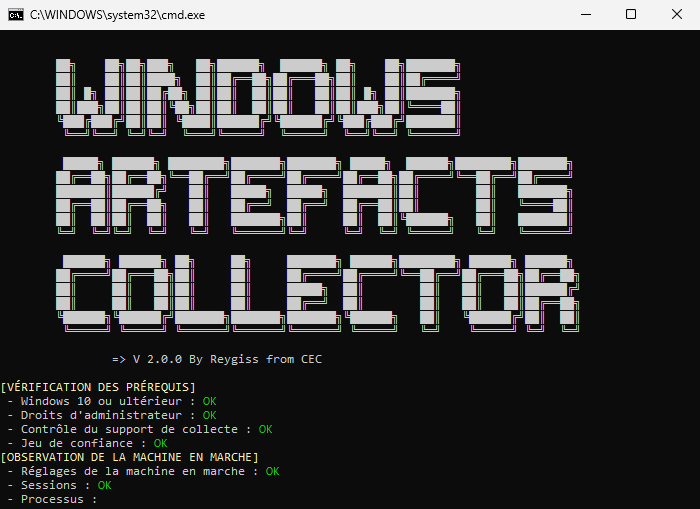
\includegraphics[width=\columnwidth,height=24mm,keepaspectratio]{../images/wac-running_FR.png}
\captionof*{figure}{\wac{} en cours de collecte.}
\end{center}

\end{document}
